%--A0 beamer slide-------------------------------------------------------------
\documentclass[final]{beamer}\usepackage[]{graphicx}\usepackage[]{color}
%% maxwidth is the original width if it is less than linewidth
%% otherwise use linewidth (to make sure the graphics do not exceed the margin)
\makeatletter
\def\maxwidth{ %
  \ifdim\Gin@nat@width>\linewidth
    \linewidth
  \else
    \Gin@nat@width
  \fi
}
\makeatother

\definecolor{fgcolor}{rgb}{0.345, 0.345, 0.345}
\newcommand{\hlnum}[1]{\textcolor[rgb]{0.686,0.059,0.569}{#1}}%
\newcommand{\hlstr}[1]{\textcolor[rgb]{0.192,0.494,0.8}{#1}}%
\newcommand{\hlcom}[1]{\textcolor[rgb]{0.678,0.584,0.686}{\textit{#1}}}%
\newcommand{\hlopt}[1]{\textcolor[rgb]{0,0,0}{#1}}%
\newcommand{\hlstd}[1]{\textcolor[rgb]{0.345,0.345,0.345}{#1}}%
\newcommand{\hlkwa}[1]{\textcolor[rgb]{0.161,0.373,0.58}{\textbf{#1}}}%
\newcommand{\hlkwb}[1]{\textcolor[rgb]{0.69,0.353,0.396}{#1}}%
\newcommand{\hlkwc}[1]{\textcolor[rgb]{0.333,0.667,0.333}{#1}}%
\newcommand{\hlkwd}[1]{\textcolor[rgb]{0.737,0.353,0.396}{\textbf{#1}}}%
\let\hlipl\hlkwb

\usepackage{framed}
\makeatletter
\newenvironment{kframe}{%
 \def\at@end@of@kframe{}%
 \ifinner\ifhmode%
  \def\at@end@of@kframe{\end{minipage}}%
  \begin{minipage}{\columnwidth}%
 \fi\fi%
 \def\FrameCommand##1{\hskip\@totalleftmargin \hskip-\fboxsep
 \colorbox{shadecolor}{##1}\hskip-\fboxsep
     % There is no \\@totalrightmargin, so:
     \hskip-\linewidth \hskip-\@totalleftmargin \hskip\columnwidth}%
 \MakeFramed {\advance\hsize-\width
   \@totalleftmargin\z@ \linewidth\hsize
   \@setminipage}}%
 {\par\unskip\endMakeFramed%
 \at@end@of@kframe}
\makeatother

\definecolor{shadecolor}{rgb}{.97, .97, .97}
\definecolor{messagecolor}{rgb}{0, 0, 0}
\definecolor{warningcolor}{rgb}{1, 0, 1}
\definecolor{errorcolor}{rgb}{1, 0, 0}
\newenvironment{knitrout}{}{} % an empty environment to be redefined in TeX

\usepackage{alltt}
\usepackage{graphicx, color}
%% maxwidth is the original width if it is less than linewidth
%% otherwise use linewidth (to make sure the graphics do not exceed the margin)
\makeatletter
\def\maxwidth{ %
  \ifdim\Gin@nat@width>\linewidth
    \linewidth
  \else
    \Gin@nat@width
  \fi
}
\makeatother

\usepackage[
  natbib = true,
    backend=bibtex,
    isbn=false,
    url=false,
    doi=false,
    eprint=false,
    sorting=none
]{biblatex}
%{\tiny
\bibliography{neuroconductor_poster.bib} % your bib file!!

%}
\renewcommand*{\bibfont}{\scriptsize}
% \newcommand{\stubber}[1]{../../results/161-413_20110710_1619_CT_2_HEAD_Head#1.png}

\usepackage{array}


\def\newblock{\hskip .11em plus .33em minus .07em} %for natbib and beamer 
\usepackage[orientation=landscape,size=a0,
            scale=1,         % font scale factor
            size=custom,
            % width=100,height=80,
            width=121,height=91, % 48 by 36
           ]{beamerposter}
\setbeamertemplate{frametitle}{
    \vspace{-5cm}\\
    \insertframetitle
}         
           
\geometry{
  hmargin=2.5cm, % little modification of margins
  vmargin = 0cm,
  head=0cm  
}
\setlength{\footskip}{0pt}

\usepackage{multirow}

\usepackage{subfig}
% 
% \usepackage{tikz}
% \usetikzlibrary{shapes,arrows}
% \usetikzlibrary{positioning}

\usepackage{adjustbox}

\usepackage[utf8]{inputenc}
%\usepackage{verbatim}

\linespread{1.15}
%
%==The poster style============================================================
\usetheme{sharelatex}

%==Title, date and authors of the poster=======================================
\title
%[Super Conference, 1 - 10 July 2013, New York, USA] % Conference
{ % Poster title
Neuroconductor: An R Platform for Medical Imaging Analysis
}
 


\author{ % Authors
John Muschelli\inst{1}, Jean-Philippe Fortin\inst{2}, Adrian Gherman\inst{1},Brian Avants\inst{2}, Brandon Whitcher\inst{3,4}, Jonathan D. Clayden\inst{5}, Brian S. Caffo\inst{1}, Ciprian M. Crainiceanu\inst{1}
}
\institute
[Johns Hopkins Bloomberg School of Public Health] % General University
{
\inst{1} Johns Hopkins Bloomberg School of Public Health, Department of
Biostatistics\\[0.3ex]
\inst{2} Perelman School of Medicine, University of Pennsylvania \;
\inst{3} Klarismo Ltd, London, UK\\[0.3ex]
\inst{4} Department of Mathematics, Imperial College London, London, UK \\[0.3ex]
\inst{5} Institute of Child Health, Developmental Imaging and Biophysics Section, University College London, UK
}

\date{\today}


\usepackage{hyperref}
\IfFileExists{upquote.sty}{\usepackage{upquote}}{}
\begin{document}

\vspace{-4cm}
\renewcommand{\thesubfigure}{\Alph{subfigure}}

\begin{frame}[fragile]
\vspace{-11cm}

\begin{table}[!htb]








%==============================================================================

\begin{minipage}{0.21\linewidth}
\section{What is Neuroconductor?}

Neuroconductor is a a centralized repository of R software dedicated to medical image analysis.

\subsection{Goals of Neuroconductor}

\begin{itemize}
\item Disseminate quickly software updates
\item Educate a large, diverse community of scientists using detailed tutorials and short courses
\item Ensure quality via automatic and manual quality controls
\item Promote the reproducibility of image data analysis
\end{itemize}

% \begin{multicols}{2}
% Left column has a list
% 
% \begin{itemize}
% \item Stuff
% \item to 
% \item List
% \end{itemize}
% \vfill
% \columnbreak
% 
% This is the right column
% 
% \end{multicols}

\subsection{Benefits of Imaging in R}

Allow medical imaging to use all R has to offer:
  
\begin{itemize}
\item Statistics and Machine Learning
\item Package versioning, testing, and distribution
\item Reproducibile reports and analyses (knitr and rmarkdown)
\item Shiny applications for the web
\end{itemize}

\section{Potential Downsides to Neuroconductor}
\begin{itemize}
\item More control over the workflow = more work (e.g.~for statisticians)
\item Users need external software (versions/installation)
\item No control over external software
  \begin{itemize}
    \item if maintainer changes something, not much recourse
  \end{itemize}
\item Need the content (buy-in from the imaging/R communities)
\end{itemize}



\begin{center}
% \includegraphics[width=0.8\linewidth]{MS_Imaging_Pipeline_Flowchart.pdf}
\end{center}
\vspace*{-0.8cm}
\section{References}
\setlength\bibitemsep{0pt}
\printbibliography[heading=none]\vspace*{-0.5cm}
\section{Sources of Funding}
{\scriptsize
The project described and data used were supported by the NIH grants R01EB012547, T32AG000247, R01NS046309, R01NS060910, R01NS085211, R01NS046309, U01NS080824, U01NS080824 and U01NS062851 and R01MH095836.
}
\end{minipage}
%\begin{minipage}{0.01\linewidth}
%\end{minipage}
\hfill{\vrule width 5pt}\hfill
%\begin{minipage}{0.01\linewidth}
%\end{minipage}
\begin{minipage}{0.40\linewidth}

\vspace{-0.5cm}
\section{Example Imaging Workflow}
\newcommand{\mywidth}{0.17}


\begin{center}
\setlength\arrayrulewidth{5pt}
\begin{tabular}{c|c}
\LARGE Typical Imaging Workflow & \LARGE Neuroconductor Workflow \\ \hline
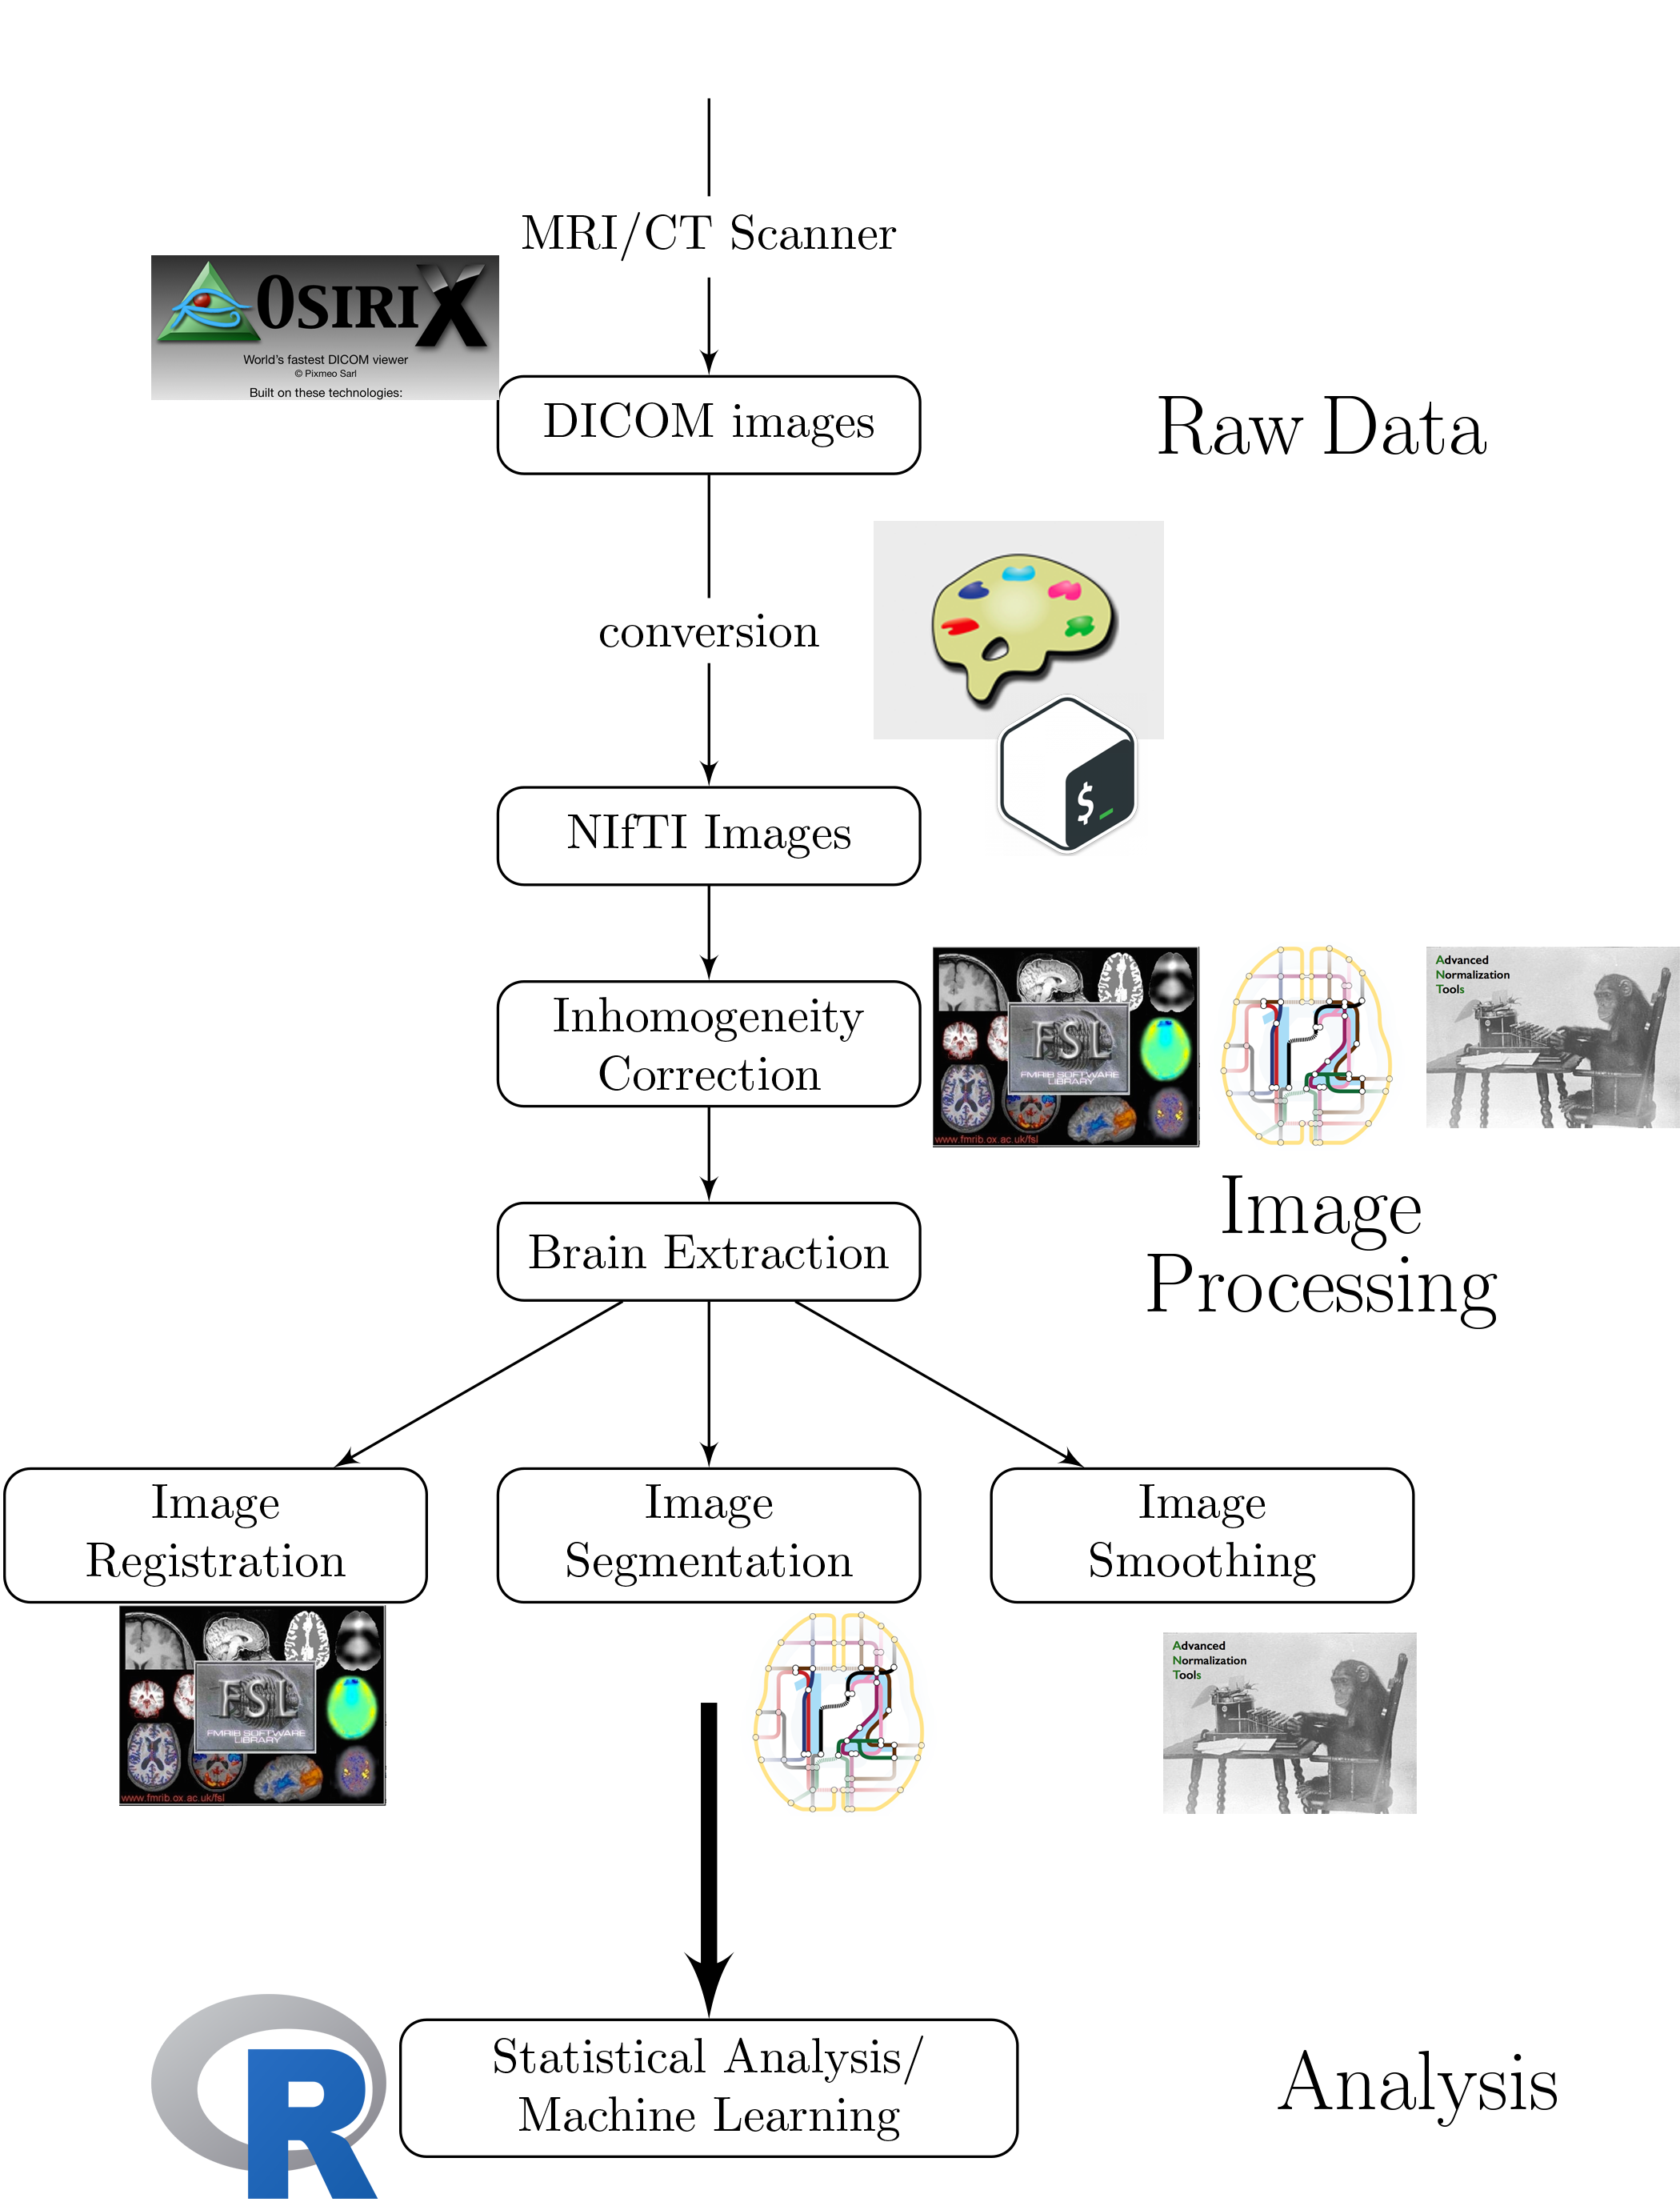
\includegraphics[clip, width=0.5\linewidth]{figures/workflow_edited_nonR.png} &
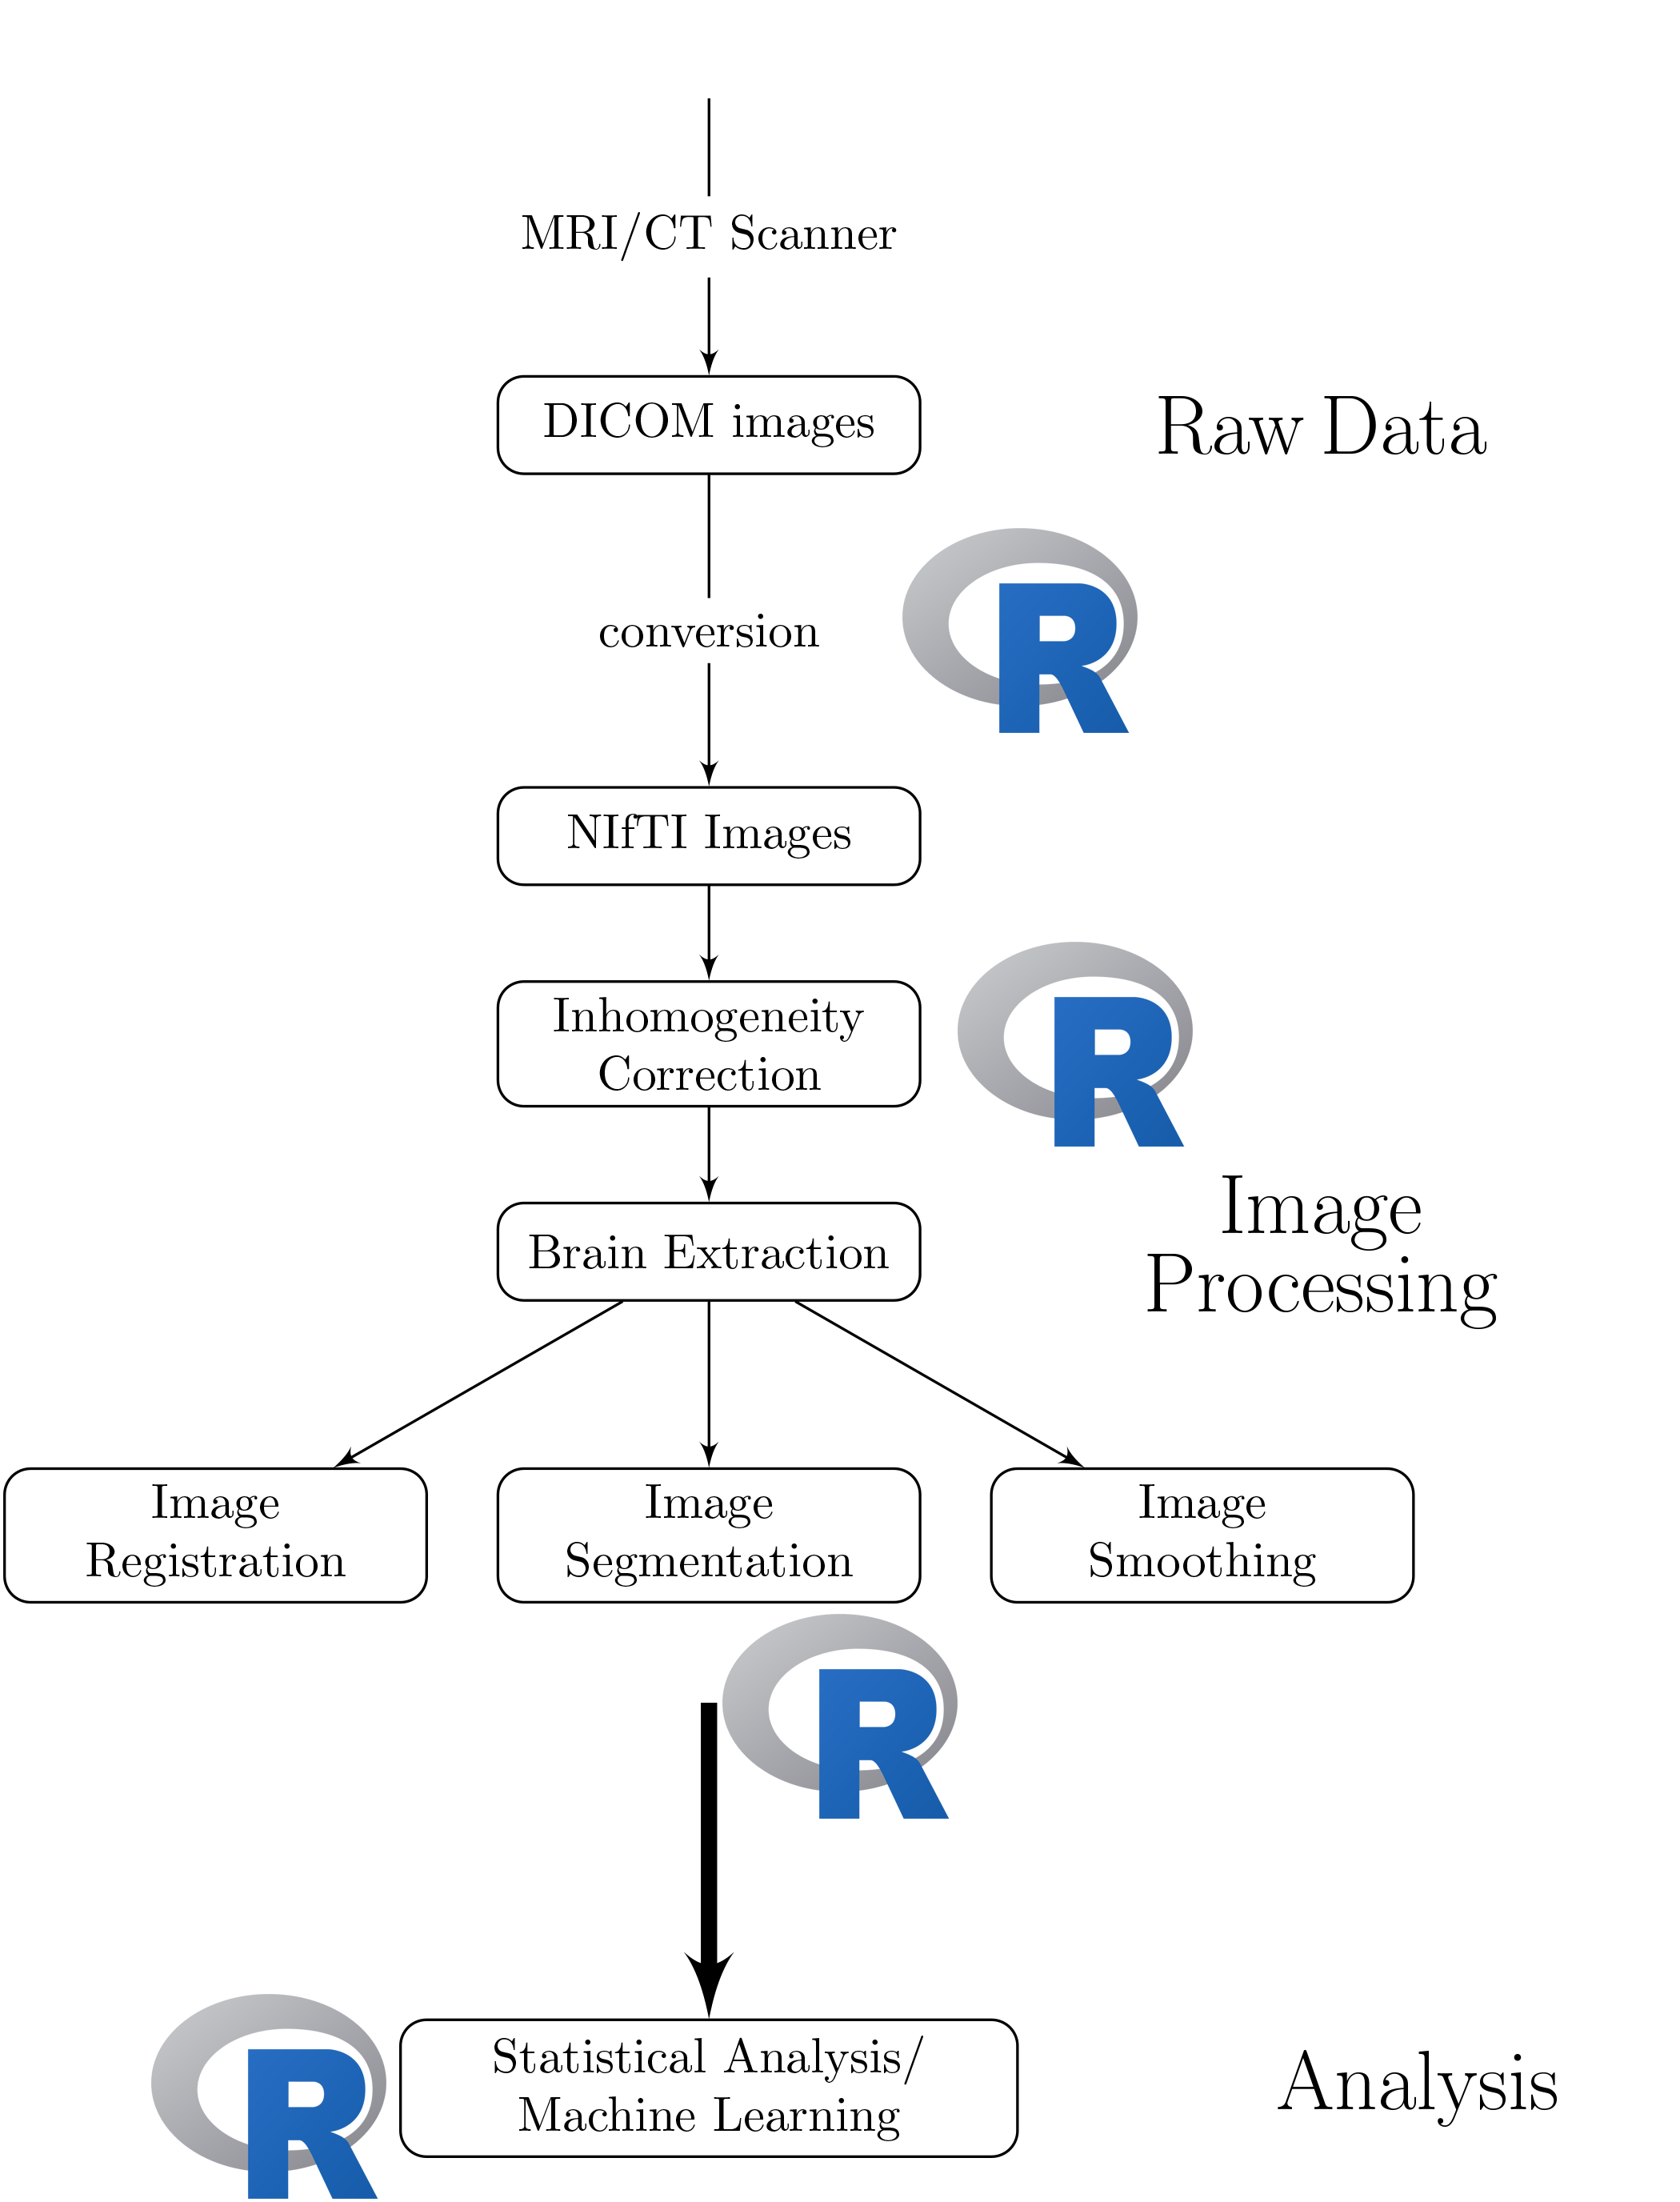
\includegraphics[clip, width=0.5\linewidth]{figures/workflow_edited_R.png}
\end{tabular}
\end{center}

\vspace*{-0.25cm}
\noindent\rule{\linewidth}{5pt}

\vspace*{1cm}
\vfill


\begin{tabular}{>{\centering}m{0.16\linewidth}>{\centering}m{0.16\linewidth}|>{\centering}m{0.16\linewidth}>{\centering}m{0.16\linewidth}|>{\centering}m{0.16\linewidth}>{\centering\arraybackslash}m{0.16\linewidth}}

\includegraphics[clip, width=5cm, keepaspectratio]{figures/Bash-new-600x600.png} 
& bash - shell scripting is usually required for command-line tools or pipelining
& 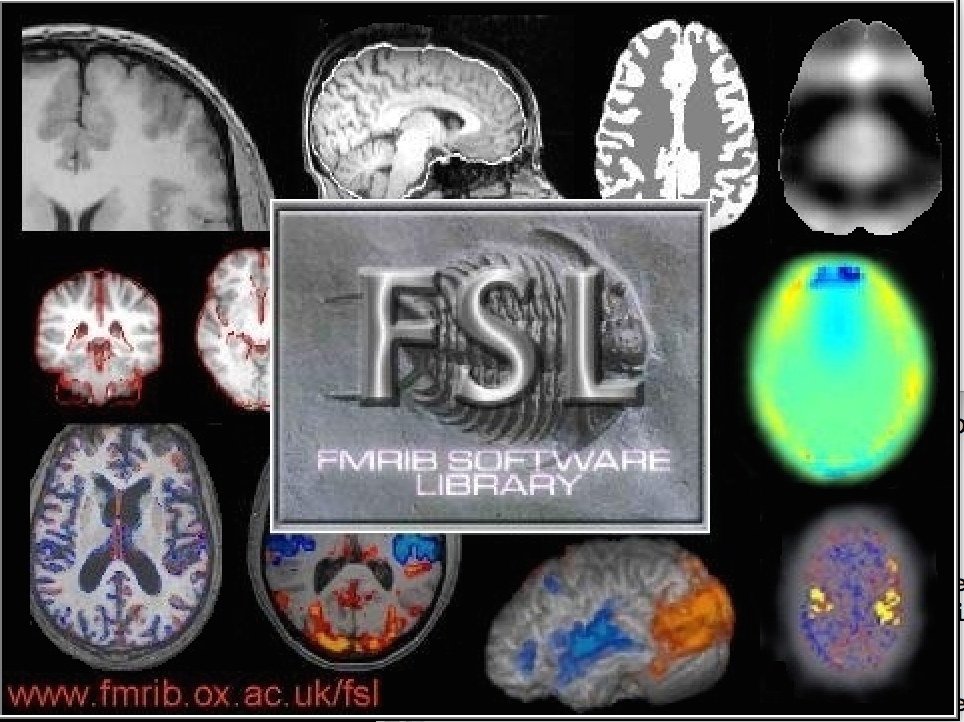
\includegraphics[clip, width=5cm, keepaspectratio]{figures/FSL.png} 
& FSL (FMRIB Software Library) - suite of neuroimaging analysis tools
& 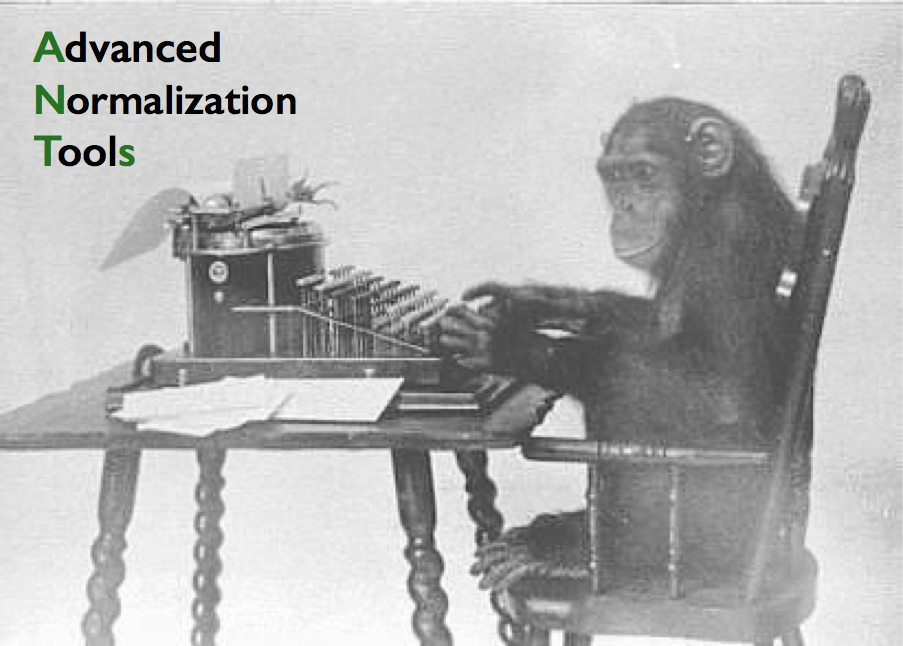
\includegraphics[clip, width=5cm, keepaspectratio]{figures/ants.png} 
& ANTs (Advanced Normalization Tools) - state-of-the-art tools for neuroimaging analysis \\
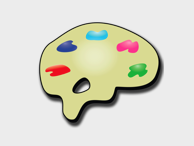
\includegraphics[clip, width=5cm, keepaspectratio]{figures/mricrogl.png}
& MRIcroGL - imaging analysis suite, with dcm2nii - DICOM to NIfTI software
& 
\includegraphics[clip, width=5cm, keepaspectratio]{figures/OsiriX.png}
& OsiriX - standalone DICOM viewer  
& 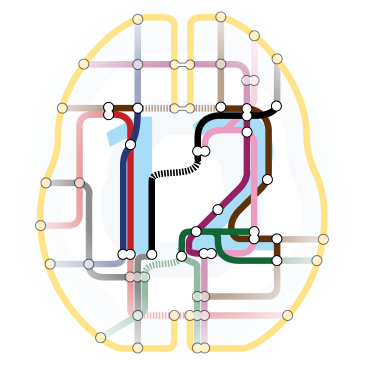
\includegraphics[clip, width=5cm, keepaspectratio]{figures/spm12.png} & SPM 12 - statistical parametric mapping, requires MATLAB (Mathworks, Natick, Massachusetts, USA) - analysis tools for PET/SPECT/fMRI
\end{tabular}


\section{Current Neuroconductor Packages}
\begin{tabular}{cc}
oro.nifti & read/write NIfTI Images \\
RNifti & read/write NIfTI Images \\
dcm2niir & convert from DICOM to NIfTI (using dcm2niix binary) \\
divest & convert from DICOM to NIfTI (using Rcpp) \citep{rcpp} \\
fslr & FSL port - preprocessing/registration/image operations \\
freesurfer & Freesurfer port - image registration/segmentation \\
ANTsR & implements ANTs in Rcpp - preprocessing/registration/image operations \\
kirby21 &  \citep{kirby} \\ 
EveTemplate  \\
malf.templates & Templates \citep{bennett2012miccai} for Multi-Atlas Label Fusion (MALF) and Skull Stripping \\
\end{tabular}




\vspace*{-0.5cm}

\vfill

\end{minipage}
\begin{minipage}{0.03\linewidth}
\end{minipage}
\hfill{\vrule width 5pt}\hfill
%\begin{minipage}{0.08\linewidth}
%\end{minipage}
\begin{minipage}{0.36\linewidth}



\vspace*{-0.65cm}
\section{Neuroconductor Developer Workflow}

\begin{center}

\includegraphics[width=0.8\linewidth]{neuroc_workflow.png}
\end{center}

\noindent\rule{\linewidth}{5pt}


% \begin{tabular}{>{\centering}m{0.245\linewidth}>{\centering}m{0.245\linewidth}|
% >{\centering}m{0.245\linewidth}>{\centering \arraybackslash}m{0.245\linewidth}}
% 
\includegraphics[clip, width=4cm, keepaspectratio]{figures/github-logo.png} 
% & GitHub  
% & 
\includegraphics[clip, width=5cm, keepaspectratio]{figures/neuroconductor_brain_type_bbg.png} 
% & R \\
% 
\includegraphics[clip, width=4cm, keepaspectratio]{figures/travis_logo.png} & Travis  &
% 
\includegraphics[clip, width=3.5cm, keepaspectratio]{figures/appveyor-logo-256.png} & AppVeyor \\
% \end{tabular}

\begin{tabular}{m{0.3\linewidth}m{0.5\linewidth}}

\includegraphics[clip, scale=0.14, keepaspectratio]{figures/github-logo.png} 
& GitHub - a online hosting service of git repositories.  All Neuroconductor packages are hosted on GitHub.  \\ \hline

\includegraphics[clip, scale=0.8, keepaspectratio]{figures/neuroconductor_brain_type_bbg.png} 
& Before uploading to GitHub, checks are performed, a confirmatory email is sent (reduce spam), and Travis/Appveyor configuration files are added \\ \hline

\includegraphics[clip, scale=0.5, keepaspectratio]{figures/travis_logo.png} & Travis CI (continuous integration) - an online service of Linux/Mac OSX virtual machines that build and check packages  \\ \hline

\includegraphics[clip, scale=0.5, keepaspectratio]{figures/appveyor-logo-256.png} & AppVeyor - a similar CI service that builds and checks packages on Windows 
\end{tabular}


\section{Conclusions}
\vspace*{-0.5cm}







\end{minipage}
\end{table}
%==============================================================================
\end{frame}




\end{document}

